\documentclass{article}
\usepackage{iclr2027_conference,times}
%%%%% NEW MATH DEFINITIONS %%%%%

\usepackage{amsmath,amsfonts,bm}

% Mark sections of captions for referring to divisions of figures
\newcommand{\figleft}{{\em (Left)}}
\newcommand{\figcenter}{{\em (Center)}}
\newcommand{\figright}{{\em (Right)}}
\newcommand{\figtop}{{\em (Top)}}
\newcommand{\figbottom}{{\em (Bottom)}}
\newcommand{\captiona}{{\em (a)}}
\newcommand{\captionb}{{\em (b)}}
\newcommand{\captionc}{{\em (c)}}
\newcommand{\captiond}{{\em (d)}}

% Highlight a newly defined term
\newcommand{\newterm}[1]{{\bf #1}}


% Figure reference, lower-case.
\def\figref#1{figure~\ref{#1}}
% Figure reference, capital. For start of sentence
\def\Figref#1{Figure~\ref{#1}}
\def\twofigref#1#2{figures \ref{#1} and \ref{#2}}
\def\quadfigref#1#2#3#4{figures \ref{#1}, \ref{#2}, \ref{#3} and \ref{#4}}
% Section reference, lower-case.
\def\secref#1{section~\ref{#1}}
% Section reference, capital.
\def\Secref#1{Section~\ref{#1}}
% Reference to two sections.
\def\twosecrefs#1#2{sections \ref{#1} and \ref{#2}}
% Reference to three sections.
\def\secrefs#1#2#3{sections \ref{#1}, \ref{#2} and \ref{#3}}
% Reference to an equation, lower-case.
\def\eqref#1{equation~\ref{#1}}
% Reference to an equation, upper case
\def\Eqref#1{Equation~\ref{#1}}
% A raw reference to an equation---avoid using if possible
\def\plaineqref#1{\ref{#1}}
% Reference to a chapter, lower-case.
\def\chapref#1{chapter~\ref{#1}}
% Reference to an equation, upper case.
\def\Chapref#1{Chapter~\ref{#1}}
% Reference to a range of chapters
\def\rangechapref#1#2{chapters\ref{#1}--\ref{#2}}
% Reference to an algorithm, lower-case.
\def\algref#1{algorithm~\ref{#1}}
% Reference to an algorithm, upper case.
\def\Algref#1{Algorithm~\ref{#1}}
\def\twoalgref#1#2{algorithms \ref{#1} and \ref{#2}}
\def\Twoalgref#1#2{Algorithms \ref{#1} and \ref{#2}}
% Reference to a part, lower case
\def\partref#1{part~\ref{#1}}
% Reference to a part, upper case
\def\Partref#1{Part~\ref{#1}}
\def\twopartref#1#2{parts \ref{#1} and \ref{#2}}

\def\ceil#1{\lceil #1 \rceil}
\def\floor#1{\lfloor #1 \rfloor}
\def\1{\bm{1}}
\newcommand{\train}{\mathcal{D}}
\newcommand{\valid}{\mathcal{D_{\mathrm{valid}}}}
\newcommand{\test}{\mathcal{D_{\mathrm{test}}}}

\def\eps{{\epsilon}}


% Random variables
\def\reta{{\textnormal{$\eta$}}}
\def\ra{{\textnormal{a}}}
\def\rb{{\textnormal{b}}}
\def\rc{{\textnormal{c}}}
\def\rd{{\textnormal{d}}}
\def\re{{\textnormal{e}}}
\def\rf{{\textnormal{f}}}
\def\rg{{\textnormal{g}}}
\def\rh{{\textnormal{h}}}
\def\ri{{\textnormal{i}}}
\def\rj{{\textnormal{j}}}
\def\rk{{\textnormal{k}}}
\def\rl{{\textnormal{l}}}
% rm is already a command, just don't name any random variables m
\def\rn{{\textnormal{n}}}
\def\ro{{\textnormal{o}}}
\def\rp{{\textnormal{p}}}
\def\rq{{\textnormal{q}}}
\def\rr{{\textnormal{r}}}
\def\rs{{\textnormal{s}}}
\def\rt{{\textnormal{t}}}
\def\ru{{\textnormal{u}}}
\def\rv{{\textnormal{v}}}
\def\rw{{\textnormal{w}}}
\def\rx{{\textnormal{x}}}
\def\ry{{\textnormal{y}}}
\def\rz{{\textnormal{z}}}

% Random vectors
\def\rvepsilon{{\mathbf{\epsilon}}}
\def\rvtheta{{\mathbf{\theta}}}
\def\rva{{\mathbf{a}}}
\def\rvb{{\mathbf{b}}}
\def\rvc{{\mathbf{c}}}
\def\rvd{{\mathbf{d}}}
\def\rve{{\mathbf{e}}}
\def\rvf{{\mathbf{f}}}
\def\rvg{{\mathbf{g}}}
\def\rvh{{\mathbf{h}}}
\def\rvu{{\mathbf{i}}}
\def\rvj{{\mathbf{j}}}
\def\rvk{{\mathbf{k}}}
\def\rvl{{\mathbf{l}}}
\def\rvm{{\mathbf{m}}}
\def\rvn{{\mathbf{n}}}
\def\rvo{{\mathbf{o}}}
\def\rvp{{\mathbf{p}}}
\def\rvq{{\mathbf{q}}}
\def\rvr{{\mathbf{r}}}
\def\rvs{{\mathbf{s}}}
\def\rvt{{\mathbf{t}}}
\def\rvu{{\mathbf{u}}}
\def\rvv{{\mathbf{v}}}
\def\rvw{{\mathbf{w}}}
\def\rvx{{\mathbf{x}}}
\def\rvy{{\mathbf{y}}}
\def\rvz{{\mathbf{z}}}

% Elements of random vectors
\def\erva{{\textnormal{a}}}
\def\ervb{{\textnormal{b}}}
\def\ervc{{\textnormal{c}}}
\def\ervd{{\textnormal{d}}}
\def\erve{{\textnormal{e}}}
\def\ervf{{\textnormal{f}}}
\def\ervg{{\textnormal{g}}}
\def\ervh{{\textnormal{h}}}
\def\ervi{{\textnormal{i}}}
\def\ervj{{\textnormal{j}}}
\def\ervk{{\textnormal{k}}}
\def\ervl{{\textnormal{l}}}
\def\ervm{{\textnormal{m}}}
\def\ervn{{\textnormal{n}}}
\def\ervo{{\textnormal{o}}}
\def\ervp{{\textnormal{p}}}
\def\ervq{{\textnormal{q}}}
\def\ervr{{\textnormal{r}}}
\def\ervs{{\textnormal{s}}}
\def\ervt{{\textnormal{t}}}
\def\ervu{{\textnormal{u}}}
\def\ervv{{\textnormal{v}}}
\def\ervw{{\textnormal{w}}}
\def\ervx{{\textnormal{x}}}
\def\ervy{{\textnormal{y}}}
\def\ervz{{\textnormal{z}}}

% Random matrices
\def\rmA{{\mathbf{A}}}
\def\rmB{{\mathbf{B}}}
\def\rmC{{\mathbf{C}}}
\def\rmD{{\mathbf{D}}}
\def\rmE{{\mathbf{E}}}
\def\rmF{{\mathbf{F}}}
\def\rmG{{\mathbf{G}}}
\def\rmH{{\mathbf{H}}}
\def\rmI{{\mathbf{I}}}
\def\rmJ{{\mathbf{J}}}
\def\rmK{{\mathbf{K}}}
\def\rmL{{\mathbf{L}}}
\def\rmM{{\mathbf{M}}}
\def\rmN{{\mathbf{N}}}
\def\rmO{{\mathbf{O}}}
\def\rmP{{\mathbf{P}}}
\def\rmQ{{\mathbf{Q}}}
\def\rmR{{\mathbf{R}}}
\def\rmS{{\mathbf{S}}}
\def\rmT{{\mathbf{T}}}
\def\rmU{{\mathbf{U}}}
\def\rmV{{\mathbf{V}}}
\def\rmW{{\mathbf{W}}}
\def\rmX{{\mathbf{X}}}
\def\rmY{{\mathbf{Y}}}
\def\rmZ{{\mathbf{Z}}}

% Elements of random matrices
\def\ermA{{\textnormal{A}}}
\def\ermB{{\textnormal{B}}}
\def\ermC{{\textnormal{C}}}
\def\ermD{{\textnormal{D}}}
\def\ermE{{\textnormal{E}}}
\def\ermF{{\textnormal{F}}}
\def\ermG{{\textnormal{G}}}
\def\ermH{{\textnormal{H}}}
\def\ermI{{\textnormal{I}}}
\def\ermJ{{\textnormal{J}}}
\def\ermK{{\textnormal{K}}}
\def\ermL{{\textnormal{L}}}
\def\ermM{{\textnormal{M}}}
\def\ermN{{\textnormal{N}}}
\def\ermO{{\textnormal{O}}}
\def\ermP{{\textnormal{P}}}
\def\ermQ{{\textnormal{Q}}}
\def\ermR{{\textnormal{R}}}
\def\ermS{{\textnormal{S}}}
\def\ermT{{\textnormal{T}}}
\def\ermU{{\textnormal{U}}}
\def\ermV{{\textnormal{V}}}
\def\ermW{{\textnormal{W}}}
\def\ermX{{\textnormal{X}}}
\def\ermY{{\textnormal{Y}}}
\def\ermZ{{\textnormal{Z}}}

% Vectors
\def\vzero{{\bm{0}}}
\def\vone{{\bm{1}}}
\def\vmu{{\bm{\mu}}}
\def\vtheta{{\bm{\theta}}}
\def\va{{\bm{a}}}
\def\vb{{\bm{b}}}
\def\vc{{\bm{c}}}
\def\vd{{\bm{d}}}
\def\ve{{\bm{e}}}
\def\vf{{\bm{f}}}
\def\vg{{\bm{g}}}
\def\vh{{\bm{h}}}
\def\vi{{\bm{i}}}
\def\vj{{\bm{j}}}
\def\vk{{\bm{k}}}
\def\vl{{\bm{l}}}
\def\vm{{\bm{m}}}
\def\vn{{\bm{n}}}
\def\vo{{\bm{o}}}
\def\vp{{\bm{p}}}
\def\vq{{\bm{q}}}
\def\vr{{\bm{r}}}
\def\vs{{\bm{s}}}
\def\vt{{\bm{t}}}
\def\vu{{\bm{u}}}
\def\vv{{\bm{v}}}
\def\vw{{\bm{w}}}
\def\vx{{\bm{x}}}
\def\vy{{\bm{y}}}
\def\vz{{\bm{z}}}

% Elements of vectors
\def\evalpha{{\alpha}}
\def\evbeta{{\beta}}
\def\evepsilon{{\epsilon}}
\def\evlambda{{\lambda}}
\def\evomega{{\omega}}
\def\evmu{{\mu}}
\def\evpsi{{\psi}}
\def\evsigma{{\sigma}}
\def\evtheta{{\theta}}
\def\eva{{a}}
\def\evb{{b}}
\def\evc{{c}}
\def\evd{{d}}
\def\eve{{e}}
\def\evf{{f}}
\def\evg{{g}}
\def\evh{{h}}
\def\evi{{i}}
\def\evj{{j}}
\def\evk{{k}}
\def\evl{{l}}
\def\evm{{m}}
\def\evn{{n}}
\def\evo{{o}}
\def\evp{{p}}
\def\evq{{q}}
\def\evr{{r}}
\def\evs{{s}}
\def\evt{{t}}
\def\evu{{u}}
\def\evv{{v}}
\def\evw{{w}}
\def\evx{{x}}
\def\evy{{y}}
\def\evz{{z}}

% Matrix
\def\mA{{\bm{A}}}
\def\mB{{\bm{B}}}
\def\mC{{\bm{C}}}
\def\mD{{\bm{D}}}
\def\mE{{\bm{E}}}
\def\mF{{\bm{F}}}
\def\mG{{\bm{G}}}
\def\mH{{\bm{H}}}
\def\mI{{\bm{I}}}
\def\mJ{{\bm{J}}}
\def\mK{{\bm{K}}}
\def\mL{{\bm{L}}}
\def\mM{{\bm{M}}}
\def\mN{{\bm{N}}}
\def\mO{{\bm{O}}}
\def\mP{{\bm{P}}}
\def\mQ{{\bm{Q}}}
\def\mR{{\bm{R}}}
\def\mS{{\bm{S}}}
\def\mT{{\bm{T}}}
\def\mU{{\bm{U}}}
\def\mV{{\bm{V}}}
\def\mW{{\bm{W}}}
\def\mX{{\bm{X}}}
\def\mY{{\bm{Y}}}
\def\mZ{{\bm{Z}}}
\def\mBeta{{\bm{\beta}}}
\def\mPhi{{\bm{\Phi}}}
\def\mLambda{{\bm{\Lambda}}}
\def\mSigma{{\bm{\Sigma}}}

% Tensor
\DeclareMathAlphabet{\mathsfit}{\encodingdefault}{\sfdefault}{m}{sl}
\SetMathAlphabet{\mathsfit}{bold}{\encodingdefault}{\sfdefault}{bx}{n}
\newcommand{\tens}[1]{\bm{\mathsfit{#1}}}
\def\tA{{\tens{A}}}
\def\tB{{\tens{B}}}
\def\tC{{\tens{C}}}
\def\tD{{\tens{D}}}
\def\tE{{\tens{E}}}
\def\tF{{\tens{F}}}
\def\tG{{\tens{G}}}
\def\tH{{\tens{H}}}
\def\tI{{\tens{I}}}
\def\tJ{{\tens{J}}}
\def\tK{{\tens{K}}}
\def\tL{{\tens{L}}}
\def\tM{{\tens{M}}}
\def\tN{{\tens{N}}}
\def\tO{{\tens{O}}}
\def\tP{{\tens{P}}}
\def\tQ{{\tens{Q}}}
\def\tR{{\tens{R}}}
\def\tS{{\tens{S}}}
\def\tT{{\tens{T}}}
\def\tU{{\tens{U}}}
\def\tV{{\tens{V}}}
\def\tW{{\tens{W}}}
\def\tX{{\tens{X}}}
\def\tY{{\tens{Y}}}
\def\tZ{{\tens{Z}}}


% Graph
\def\gA{{\mathcal{A}}}
\def\gB{{\mathcal{B}}}
\def\gC{{\mathcal{C}}}
\def\gD{{\mathcal{D}}}
\def\gE{{\mathcal{E}}}
\def\gF{{\mathcal{F}}}
\def\gG{{\mathcal{G}}}
\def\gH{{\mathcal{H}}}
\def\gI{{\mathcal{I}}}
\def\gJ{{\mathcal{J}}}
\def\gK{{\mathcal{K}}}
\def\gL{{\mathcal{L}}}
\def\gM{{\mathcal{M}}}
\def\gN{{\mathcal{N}}}
\def\gO{{\mathcal{O}}}
\def\gP{{\mathcal{P}}}
\def\gQ{{\mathcal{Q}}}
\def\gR{{\mathcal{R}}}
\def\gS{{\mathcal{S}}}
\def\gT{{\mathcal{T}}}
\def\gU{{\mathcal{U}}}
\def\gV{{\mathcal{V}}}
\def\gW{{\mathcal{W}}}
\def\gX{{\mathcal{X}}}
\def\gY{{\mathcal{Y}}}
\def\gZ{{\mathcal{Z}}}

% Sets
\def\sA{{\mathbb{A}}}
\def\sB{{\mathbb{B}}}
\def\sC{{\mathbb{C}}}
\def\sD{{\mathbb{D}}}
% Don't use a set called E, because this would be the same as our symbol
% for expectation.
\def\sF{{\mathbb{F}}}
\def\sG{{\mathbb{G}}}
\def\sH{{\mathbb{H}}}
\def\sI{{\mathbb{I}}}
\def\sJ{{\mathbb{J}}}
\def\sK{{\mathbb{K}}}
\def\sL{{\mathbb{L}}}
\def\sM{{\mathbb{M}}}
\def\sN{{\mathbb{N}}}
\def\sO{{\mathbb{O}}}
\def\sP{{\mathbb{P}}}
\def\sQ{{\mathbb{Q}}}
\def\sR{{\mathbb{R}}}
\def\sS{{\mathbb{S}}}
\def\sT{{\mathbb{T}}}
\def\sU{{\mathbb{U}}}
\def\sV{{\mathbb{V}}}
\def\sW{{\mathbb{W}}}
\def\sX{{\mathbb{X}}}
\def\sY{{\mathbb{Y}}}
\def\sZ{{\mathbb{Z}}}

% Entries of a matrix
\def\emLambda{{\Lambda}}
\def\emA{{A}}
\def\emB{{B}}
\def\emC{{C}}
\def\emD{{D}}
\def\emE{{E}}
\def\emF{{F}}
\def\emG{{G}}
\def\emH{{H}}
\def\emI{{I}}
\def\emJ{{J}}
\def\emK{{K}}
\def\emL{{L}}
\def\emM{{M}}
\def\emN{{N}}
\def\emO{{O}}
\def\emP{{P}}
\def\emQ{{Q}}
\def\emR{{R}}
\def\emS{{S}}
\def\emT{{T}}
\def\emU{{U}}
\def\emV{{V}}
\def\emW{{W}}
\def\emX{{X}}
\def\emY{{Y}}
\def\emZ{{Z}}
\def\emSigma{{\Sigma}}

% entries of a tensor
% Same font as tensor, without \bm wrapper
\newcommand{\etens}[1]{\mathsfit{#1}}
\def\etLambda{{\etens{\Lambda}}}
\def\etA{{\etens{A}}}
\def\etB{{\etens{B}}}
\def\etC{{\etens{C}}}
\def\etD{{\etens{D}}}
\def\etE{{\etens{E}}}
\def\etF{{\etens{F}}}
\def\etG{{\etens{G}}}
\def\etH{{\etens{H}}}
\def\etI{{\etens{I}}}
\def\etJ{{\etens{J}}}
\def\etK{{\etens{K}}}
\def\etL{{\etens{L}}}
\def\etM{{\etens{M}}}
\def\etN{{\etens{N}}}
\def\etO{{\etens{O}}}
\def\etP{{\etens{P}}}
\def\etQ{{\etens{Q}}}
\def\etR{{\etens{R}}}
\def\etS{{\etens{S}}}
\def\etT{{\etens{T}}}
\def\etU{{\etens{U}}}
\def\etV{{\etens{V}}}
\def\etW{{\etens{W}}}
\def\etX{{\etens{X}}}
\def\etY{{\etens{Y}}}
\def\etZ{{\etens{Z}}}

% The true underlying data generating distribution
\newcommand{\pdata}{p_{\rm{data}}}
% The empirical distribution defined by the training set
\newcommand{\ptrain}{\hat{p}_{\rm{data}}}
\newcommand{\Ptrain}{\hat{P}_{\rm{data}}}
% The model distribution
\newcommand{\pmodel}{p_{\rm{model}}}
\newcommand{\Pmodel}{P_{\rm{model}}}
\newcommand{\ptildemodel}{\tilde{p}_{\rm{model}}}
% Stochastic autoencoder distributions
\newcommand{\pencode}{p_{\rm{encoder}}}
\newcommand{\pdecode}{p_{\rm{decoder}}}
\newcommand{\precons}{p_{\rm{reconstruct}}}

\newcommand{\laplace}{\mathrm{Laplace}} % Laplace distribution

\newcommand{\E}{\mathbb{E}}
\newcommand{\Ls}{\mathcal{L}}
\newcommand{\R}{\mathbb{R}}
\newcommand{\emp}{\tilde{p}}
\newcommand{\lr}{\alpha}
\newcommand{\reg}{\lambda}
\newcommand{\rect}{\mathrm{rectifier}}
\newcommand{\softmax}{\mathrm{softmax}}
\newcommand{\sigmoid}{\sigma}
\newcommand{\softplus}{\zeta}
\newcommand{\KL}{D_{\mathrm{KL}}}
\newcommand{\Var}{\mathrm{Var}}
\newcommand{\standarderror}{\mathrm{SE}}
\newcommand{\Cov}{\mathrm{Cov}}
% Wolfram Mathworld says $L^2$ is for function spaces and $\ell^2$ is for vectors
% But then they seem to use $L^2$ for vectors throughout the site, and so does
% wikipedia.
\newcommand{\normlzero}{L^0}
\newcommand{\normlone}{L^1}
\newcommand{\normltwo}{L^2}
\newcommand{\normlp}{L^p}
\newcommand{\normmax}{L^\infty}

\newcommand{\parents}{Pa} % See usage in notation.tex. Chosen to match Daphne's book.

\DeclareMathOperator*{\argmax}{arg\,max}
\DeclareMathOperator*{\argmin}{arg\,min}

\DeclareMathOperator{\sign}{sign}
\DeclareMathOperator{\Tr}{Tr}
\let\ab\allowbreak

\usepackage{hyperref}
\usepackage{url}
\usepackage{booktabs}
\usepackage{amsmath,amssymb,amsthm}
\usepackage{graphicx}
\usepackage{xcolor}
\usepackage{multirow}

\usepackage{microtype}

\newtheorem{proposition}{Proposition}
\newcommand{\ident}{\mathrm{ident}}
\newcommand{\invert}{\mathrm{invert}}
\newcommand{\recover}{\mathrm{recover}}
\newcommand{\pihalf}{$\pi_{0.5}$}
\newcommand{\ph}{\textsuperscript{\dag}}

\title{What a Robot Can Measure, It Can Undo:\\ Separating Invertible Nuisances from Policy Failures at Deployment}

\author{Anonymous authors\\ Paper under double-blind review}

\begin{document}
\maketitle

\begin{abstract}
Robotic manipulation policies often degrade under deployment shifts that alter the observation while leaving the
underlying task unchanged. We study whether such shifts can be identified and corrected before rollout without
modifying the policy. Using joint encoders, kinematics, and the robot silhouette, we define a policy-free
recoverability score, $\recover=\ident\times\invert$, that measures whether a nuisance can be identified from
self-observation and whether its estimated inverse can reconstruct the training observation. With all constants fixed
before evaluation, the score predicts which failed episodes are repaired on two held-out policy families (AUROC 0.81
and 0.68), whereas perturbation category is near chance (0.52 and 0.47). The same measurements support training-free
correction: servoing to the training initial pose repairs 47/47 failures on three untuned suites, and marker-free
camera estimation followed by depth reprojection repairs 61/100 camera failures across four suites
($p=1.3\times10^{-6}$). A static silhouette test avoids unnecessary calibration motion and produces a net improvement
on held-out $\pi_{0.5}$ ($p=0.013$). Finally, among 100 camera-shift failures of the development policy, only one
persists after perfect restoration to the training view; the remainder are attributable to pose-estimation error or
missing visual coverage.
\end{abstract}

\section{Introduction}

Vision-language-action (VLA) policies are commonly trained and evaluated under a fixed sensing and robot configuration,
yet deployment inevitably introduces changes in camera pose, robot initialization, illumination, and other aspects of
the observation process. LIBERO-Plus \citep{liberoplus} makes the resulting robustness gap explicit: camera and
initial-pose perturbations can reduce task success from roughly 90\% to below 30\%. Existing approaches generally respond
to this problem in one of two ways. Some attempt to make the policy itself more robust, whereas others place a corrective
mechanism around a frozen policy, for example by restoring corrupted streams \citep{rightstream,crt,byovla}, synthesizing
a canonical view \citep{anycamvla,vistabot,gsvla}, or estimating camera state within a retrained policy
\citep{fixedtofree}.

This paper considers a different but complementary question: when a policy fails after deployment, to what extent is the
failure actually attributable to the policy? Some deployment shifts alter the observation process while leaving the
underlying task unchanged. In such cases, retraining is not necessarily the appropriate response. If the shift can be
estimated from measurements available to the robot and its effect on the observation can be inverted, then the original
policy may remain adequate once the training observation is approximately restored.

A perturbation category alone does not determine whether such a correction is possible. Two conditions may both be
described as camera shifts while differing substantially in what can be recovered. A moderate orbit around the scene may
retain most of the training view, whereas a camera that turns away from the workspace may remove information that no
single-view transformation can reconstruct. Repairability therefore depends on two distinct questions: whether the
deployment nuisance can be identified from available measurements, and whether correcting that nuisance preserves
enough information to reconstruct the observation distribution seen during training.

We use the robot itself as the calibration target. Joint encoders provide the robot configuration, while the kinematic
model predicts where the robot body should appear in the image under a candidate camera pose. These self-observations
are available independently of the surrounding scene and the policy. They allow the system to estimate deployment
nuisances, assess whether a correction is likely to be useful, apply the corresponding inverse transformation, and
verify geometric consistency afterward. The policy remains frozen throughout.

The resulting method is organized around a policy-free \emph{recoverability score} that separates
\emph{identifiability} from \emph{invertibility}. We evaluate whether this score transfers across policy families,
whether self-measurement can support useful corrections for initial-pose and camera shifts, and whether residual failures
can be localized to sensing, lost visual coverage, or the policy itself.

Our contributions are fourfold. First, we introduce a recoverability score that is fixed before held-out evaluation and
predicts which failed episodes are repairable on two unseen policy families (Sec.~\ref{sec:score}). Second, we show that
self-measurement supports two training-free corrections: proprioceptive servoing to the training initial pose and
marker-free camera calibration from the robot silhouette followed by depth-based reprojection
(Sec.~\ref{sec:undo}). Third, we derive a static silhouette test that determines whether active camera calibration is
necessary, thereby reducing failures caused by the calibration motion itself (Sec.~\ref{sec:cost}). Finally, we use an
interventional attribution procedure to distinguish calibration error, irreversible loss of view, and residual policy
failure (Sec.~\ref{sec:ladder}), and we separately examine whether the policy's own action field provides a useful
diagnostic signal (Sec.~\ref{sec:policy}).

\begin{figure}[!t]
\centering
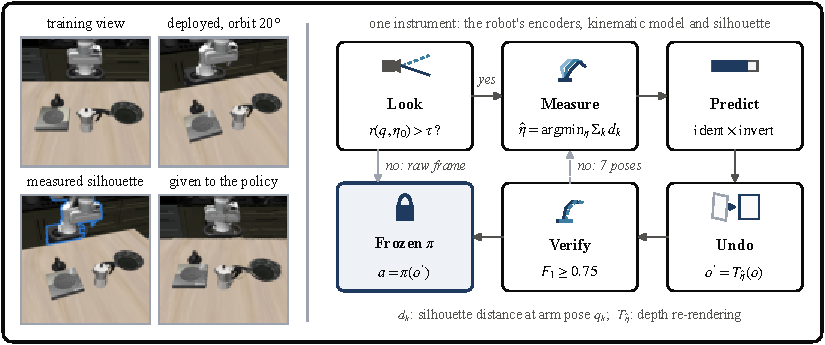
\includegraphics[width=0.97\linewidth]{figs_v2/fig2_method.pdf}
\caption{Overview of the deployment-time wrapper. The robot first checks whether the current observation is consistent with the training camera, measures the nuisance only when necessary, predicts whether the shift is recoverable, applies the corresponding inverse transformation, and verifies the result before handing the corrected observation to the frozen policy.}
\label{fig:teaser}
\end{figure}

\section{Related work}
\label{sec:related}

Several recent methods address deployment shift while leaving the underlying VLA frozen. Restoring the Right Stream
\citep{rightstream} applies training-free stream restoration on LIBERO-Plus; BYOVLA \citep{byovla} edits
task-irrelevant regions, CRT \citep{crt} restores corrupted inputs, and ProbeAct \citep{probeact} modifies actions
rather than observations. These approaches establish that useful adaptation can occur outside the policy itself. Our
focus is narrower: rather than assuming that a correction should be applied, we ask whether the observed shift is
measurable and whether the corresponding inverse can recover the training observation.

Camera variation has also been addressed directly through view synthesis and calibration. AnyCamVLA
\citep{anycamvla} re-renders observations for a frozen VLA using camera pose obtained from fiducial markers, while
VistaBot \citep{vistabot} and GS-VLA \citep{gsvla} learn view synthesis and CamVLA \citep{fixedtofree} predicts camera
state inside a retrained policy. Independently, render-and-compare robot pose estimation
\citep{dream,robopose,ctrnet,gisr} and mask-based hand--eye calibration \citep{easyhec,easyhecpp} provide established
ways to recover camera geometry from the robot body, and related procedures have been used to calibrate DROID
\citep{droid} offline from robot masks \citep{caliball,poseddroid}. We do not introduce a new reprojection or calibration
algorithm. Instead, we use self-calibration as a deployment-time measurement and connect the conditioning of that
measurement, together with retained visual coverage, to the downstream probability of successful correction.
A separate line of work attempts to predict or detect failures. RoboART \citep{roboart} estimates degradation under
visual shift using policy representations, while runtime monitors
\citep{sentinel,faildetect,safevla,fiper,actprobe,triinfo} inspect statistics of policy outputs. Our recoverability score
differs in that it predicts whether an observation-level correction is feasible without querying the policy. Conceptually,
this connects to task-relevant distribution shift \citep{farid}, identifiability in test-time adaptation
\citep{ttaident}, selective adaptation \citep{selectivetta}, and learned canonicalization \citep{kaba}. These works
motivate our broader view that deployment robustness depends not only on the policy but also on whether the deployment
shift itself is observable and reversible.

\section{Recoverability from Self-Measurement}

\label{sec:method}

Let $o=g(s;\eta)$ denote the observation of state $s$ under nuisance parameters $\eta$, with $\eta_0$ denoting the
training setup. We call a nuisance \emph{invertible} at $\eta$ if a transformation $T_\eta$, computed from measurements
available to the robot, approximately recovers the corresponding training observation,
$T_\eta(g(s;\eta))\approx g(s;\eta_0)$, over the task-relevant states. Figure~\ref{fig:teaser} summarizes the
resulting pipeline.

The first stage estimates the deployment nuisance from robot self-observations $z$. These observations include joint
readings, arm silhouettes at selected robot configurations, color statistics on robot links, and image noise measured on
robot pixels. For camera shifts, the estimated pose $\hat\eta_c$ is obtained by minimizing a silhouette Chamfer term and
a projected-size term over multiple robot configurations, using a coarse orbit search followed by cross-entropy
refinement and depth ICP. The estimate is accepted only when it improves the objective relative to the training pose by
a fixed factor. Illumination and noise are estimated from robot pixels using, respectively, an affine color model and a
noise-floor estimate.

We then quantify whether the estimated nuisance is both measurable and correctable:

\[
\recover(\eta)=
\underbrace{\min\!\left(1,\frac{\sigma_{\min}(J_\eta)}
{\sigma_{\min}(J_{\eta_0})}\right)}_{\ident}
\times
\underbrace{\invert(\eta)}_{\text{recoverable information}},\qquad
J_\eta=\partial z/\partial\eta .
\]
The identifiability term compares how strongly the robot body constrains the nuisance at deployment with how strongly it
does so in the training configuration. The invertibility term depends on the nuisance channel. For camera shifts, it is
the fraction of training-view pixels that can be populated by reprojection from the deployed camera, which we refer to
as \emph{coverage}. For illumination, it is based on an affine-invariant shading statistic on the robot links; for
sensor noise, it is the fraction of measured added noise removed by the denoiser. Joint offsets are assigned
$\invert=1$, while scene-content changes are assigned $\invert=0$ because the wrapper has no corresponding inverse.
All thresholds and constants are fixed before evaluating the held-out policy families.

When a nuisance is deemed correctable, the corresponding inverse is applied before the frozen policy receives the
observation. Initial-joint offsets are corrected by servoing the robot to the training configuration. Camera shifts are
corrected by reprojecting the RGB-D observation into the training camera using $\hat\eta_c$ and z-buffering.
Illumination and noise are corrected using the fitted channel-specific inverse models. Camera correction is additionally
checked for geometric self-consistency: the observed robot silhouette is warped using the estimated camera geometry and
compared with the silhouette predicted from forward kinematics in the training view. If agreement falls below the fixed
threshold $F_1<0.75$, the system repeats calibration using seven poses and retains the estimate with higher silhouette
agreement.

\subsection{Theoretical Properties}

\label{sec:theory}

The following propositions formalize the two quantities used by the score and two diagnostic tests used later.
Proofs are in Appendix~\ref{app:proofs}. Let $z(q,\eta)$ denote a self-observation at joint configuration $q$, with
the robot selecting configurations $q_1,\dots,q_K$.

\begin{proposition}[measurement error from the body alone]
\label{prop:cr}
If $J = \partial [z(q_1,\eta); \dots; z(q_K,\eta)] / \partial\eta$ has full column rank and the self-observations
carry independent noise of variance $\sigma^2$, every unbiased estimator satisfies $\mathbb{E}\|\hat\eta - \eta\|^2 \ge
\sigma^2\,\mathrm{tr}\big((J^\top J)^{-1}\big) \ge \sigma^2 / \sigma_{\min}(J)^2$, and adding a pose never lowers
$\sigma_{\min}(J)$.
\end{proposition}
This is why $\ident$ is a ratio of smallest singular values. Measured on 8 camera tasks: $\sigma_{\min}$ rises from
1.04 to 3.58 from one pose to seven, and the calibration error falls from 0.54 to 0.07 cm.

\begin{proposition}[what re-rendering can restore]
\label{prop:cov}
Let $V$ be the training-view pixels visible from the deployed camera, coverage $c = |V|/|\Omega|$. Any restoration
$\hat o$ computed from the deployed frame alone satisfies $\mathbb{E}\,\|\hat o - o_{\mathrm{train}}\|_1 \ge
(1-c)\,e_{\mathrm{prior}} + c\,e_V$, with $e_{\mathrm{prior}}$ the best prior fill and $e_V$ the resampling error on
seen pixels: no single-view re-rendering wrapper, ours or any other, restores what the deployed camera did not see.
\end{proposition}
Coverage is therefore an upper bound on the camera $\invert$, not a heuristic.

\begin{proposition}[a motion-free test for ``the camera moved'']
\label{prop:static}
If the camera is at $\eta_0$ and the body model is exact, the residual $r(q) = d\big(z_{\mathrm{obs}}(q),\,
z(q,\eta_0)\big)$ is zero up to noise; a residual above the noise floor proves $\eta \ne \eta_0$. One pose does not
identify $\eta$, but it decides whether identification is needed.
\end{proposition}

\begin{proposition}[a diverging opening field has no sub-goal]
\label{prop:div}
Let the opening action near $p_0$ be $a(p) = a_0 + A\,(p - p_0)$. Triangulating a sub-goal from probes assumes
$A = -\lambda I \prec 0$. If the symmetric part of $A$ is positive definite, the least-squares point is a source the
field flows away from, and its residual carries no information about miscalibration.
\end{proposition}

\section{Experiments}

We evaluate on the four LIBERO-Plus suites \citep{liberoplus}. OpenVLA-OFT \citep{oft}, using its per-suite
checkpoints, serves as the development policy family. After fixing all method constants, we evaluate two held-out
families: $\pi_{0.5}$ \citep{pi05} and base OpenVLA \citep{openvla}. Base OpenVLA is substantially weaker in this
setting, with 0.19 success over 210 LIBERO-Plus tasks. Unless otherwise stated, comparisons are paired by task and seed
and analyzed using exact McNemar tests on discordant pairs. Simulator segmentation and depth serve as proxies for a
robot segmenter and an RGB-D sensor; Sec.~\ref{sec:limits} examines the implications of this assumption. Analyses
designed after the primary experiments are marked \ph. Appendix~\ref{app:prereg} lists the tests that were registered
before their evaluation data were generated, together with all outcomes.

\subsection{Predicting Repairability}

\label{sec:score}

\begin{table}[!t]
\centering\small
\caption{Policy-free prediction of which raw failures are repaired. Constants are fixed before held-out evaluation; the initial three-task test is in Appendix~\ref{app:extra}.}
\label{tab:score}
\resizebox{\linewidth}{!}{%
\begin{tabular}{lcccc}
\toprule
& units (raw failures) & repaired & AUROC, score & AUROC, category label \\
\midrule
OpenVLA-OFT (development), ten base tasks & 65 & 37 & 0.823 [0.71, 0.92] & 0.518 \\
$\pi_{0.5}$ (held out), ten base tasks & 72 & 37 & \textbf{0.809} [0.69, 0.91] & 0.515 \\
base OpenVLA (held out), four base tasks & 60 & 24 & \textbf{0.675} [0.52, 0.82] & 0.472 \\
pooled & 197 & 98 & 0.763 [0.69, 0.83] & 0.510 \\
\bottomrule
\end{tabular}}
\end{table}

The score transfers to both held-out policy families, whereas the perturbation-category baseline remains close to chance
(Table~\ref{tab:score}). This difference is particularly clear for $\pi_{0.5}$. Identifiability alone reaches only
0.53 AUROC because some camera configurations remain measurable even though too little of the training view survives for
reprojection to be effective. The six look-away conditions illustrate this distinction: they receive recoverability
scores between 0.14 and 0.49, and none is repaired. Across 264 camera placements and 200 logged LIBERO-Plus camera tasks
containing 88 raw failures, empirical repair probability increases from 14\% to 88\% as the predicted camera term
increases (AUROC 0.78 [0.67, 0.88]; Fig.~\ref{fig:envelope}).

\begin{figure}[!t]
\centering
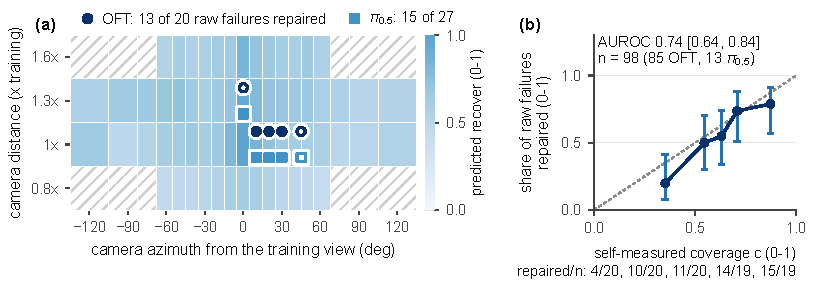
\includegraphics[width=\linewidth]{figs/envelope.pdf}
\caption{Recoverability under camera shift. Left: policy-free score over 264 placements. Middle: score under look-away rotation. Right: predicted coverage versus observed repair on 88 raw failures.}
\label{fig:envelope}
\end{figure}

The weaker base OpenVLA policy also reveals an important evaluation confound. Five of its 24 episodes counted as
``repaired'' succeed even though no correction channel is applied, compared with 0/37 for OFT and 1/37 for
$\pi_{0.5}$. In these episodes, the arm motion used for calibration changes the initial condition sufficiently to alter
the outcome of a fragile policy. Four of the five cases occur under background perturbations, for which the score
correctly assigns $\invert=0$ but is nevertheless penalized by the binary repair label. Excluding these motion-induced
successes produces similar AUROC values across the three policy families: 0.823, 0.831, and 0.816. The calibration-motion
effect is examined directly in Sec.~\ref{sec:cost}.

\subsection{Correction Performance}

\label{sec:undo}

\begin{table}[!t]
\centering\small
\caption{Paired correction results. ``rec.'' denotes repaired raw failures and ``broken'' denotes raw successes lost after wrapping.}
\label{tab:suites}
\resizebox{\linewidth}{!}{%
\begin{tabular}{llcccccc}
\toprule
policy & suite & \multicolumn{3}{c}{joint offset} & \multicolumn{3}{c}{camera} \\
& & raw $\to$ wrapped & rec. & broken & raw $\to$ wrapped & rec. & broken \\
\midrule
OFT & spatial & 0.25 $\to$ 0.95 & 15/15 & 1/5 & 0.90 $\to$ 0.88 & 3/6 & 4/54 \\
OFT & object & 0.20 $\to$ 1.00 & 16/16 & 0/4 & 0.42 $\to$ \textbf{0.75} & 26/35 & 6/25 \\
OFT & goal & 0.20 $\to$ 1.00 & 16/16 & 0/4 & 0.67 $\to$ 0.78 & 12/20 & 5/40 \\
OFT & libero-10 & 0.33 $\to$ 0.90 & & & 0.35 $\to$ \textbf{0.63} & 20/39 & 3/21 \\
$\pi_{0.5}$ & libero-10 & 0.37 $\to$ \textbf{0.90} & 16/19 & 0/11 & 0.20 $\to$ 0.37 & 7/24 & 2/6 \\
\bottomrule
\end{tabular}}
\end{table}

The initial-pose correction is the most reliable intervention in our evaluation. Across the three untuned suites,
servoing the robot back to the training configuration repairs all 47 raw failures while breaking 1 of 13 raw successes
($p=3\times10^{-13}$). The same correction transfers to held-out $\pi_{0.5}$, where it repairs 16 of 19 failures and
breaks none.

Camera correction is more difficult because accurate pose estimation is not sufficient when the deployed view has lost
task-relevant information. Across the four OFT suites, the camera wrapper repairs 61 of 100 raw failures while breaking
18 of 140 raw successes ($p=1.3\times10^{-6}$). The improvement is significant on
\texttt{libero\_object} ($p=5\times10^{-4}$) and \texttt{libero\_10}. On
\texttt{libero\_spatial}, by contrast, the raw checkpoint already succeeds on 90\% of shifted observations, leaving
little room for improvement and making the wrapper approximately neutral. For $\pi_{0.5}$, one rollout per task does
not provide sufficient evidence for the camera channel ($p=0.18$). Repeating the same 30 camera tasks three times yields
90 paired episodes, of which 21 are repaired and 8 regress, increasing success from 0.22 to 0.37
($p=0.024$).

\begin{figure}[!t]
\centering
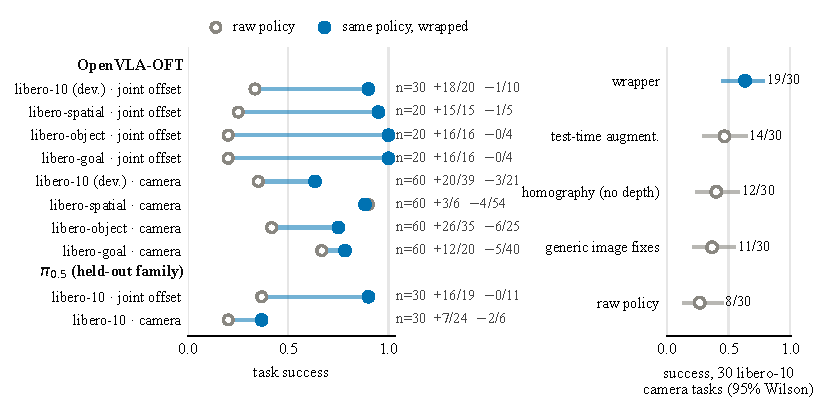
\includegraphics[width=\linewidth]{figs/_unused/paired_results.pdf}
\caption{Paired raw-versus-wrapped outcomes (left) and camera-correction baselines on 30 \texttt{libero\_10} tasks (right).}
\label{fig:paired}
\end{figure}

The baseline comparison helps separate the value of explicit geometric measurement from generic image preprocessing.
White balancing, CLAHE, and denoising provide only modest gains, while homography-based reprojection using the measured
camera pose remains limited because it does not account for scene depth (exact values are reported in Appendix~\ref{app:baselines}). Test-time
augmentation is the strongest baseline in the 30-task subset and introduces no regressions there. Nevertheless, across
150 camera tasks from three suites, the proposed wrapper outperforms augmentation on 46 tasks and underperforms on 13
($p<10^{-4}$). Augmentation alone also fails to improve over the raw policy on
\texttt{libero\_object} or \texttt{libero\_goal}.

\subsection{Calibration Overhead and Selective Measurement}

\label{sec:cost}

\begin{figure}[!t]
\centering
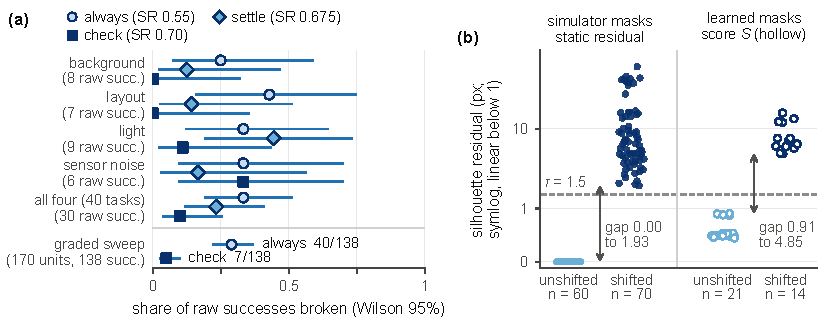
\includegraphics[width=0.92\linewidth]{figs/harm.pdf}
\caption{Calibration motion can harm $\pi_{0.5}$. Left: regressions under three measurement strategies. Right: the rest-pose silhouette residual used to decide whether active calibration is needed.}
\label{fig:harm}
\end{figure}

Active camera calibration is not itself cost-free because the measurement procedure moves the arm before the episode
begins. This interaction is negligible for some policies but substantial for held-out $\pi_{0.5}$. In the ten-task
sweep, the measuring wrapper repairs 44 of 82 raw failures but also breaks 45 of 158 raw successes. Forty of those
regressions occur in conditions where no camera correction is ultimately applied, indicating that the calibration
trajectory rather than the image transformation is responsible. After calibration, the arm is typically displaced by
10--25 mm from its initial configuration and is still moving at 0.19 rad/s. In contrast, rerunning the raw policy with
identical seeds changes the outcome on 0 of 20 tasks, which makes stochastic policy variation an unlikely explanation.
Proposition~\ref{prop:static} motivates a simple way to avoid unnecessary calibration motion. Before moving the arm, the
robot compares its observed rest-pose silhouette with the silhouette predicted under the training camera. Active
measurement is performed only when the residual exceeds the fixed noise threshold. In the logged data, this test
separates shifted from unshifted cases cleanly. Applied to the complete sweep, it reduces the number of regressions from
40 to 7 while retaining 21 of the 25 repairs obtained by always measuring. Relative to the always-measure variant, the
selective strategy improves 41 units and worsens 12 ($p=8\times10^{-5}$). Relative to the raw policy, it yields 21
repairs and 7 regressions ($p=0.013$). These results indicate that the decision to measure can be as important as the
measurement procedure itself when the policy is sensitive to its initial physical state.

\subsection{Failure Attribution}

\label{sec:ladder}

To determine why a corrected episode can still fail, we use an interventional attribution procedure\ph. For each task
and seed, we evaluate four increasingly informative conditions: the raw observation, correction using the measured camera
pose, correction using the simulator's true camera pose, and a perfect render from the training camera. A raw failure is
assigned to the first intervention that restores success. This construction separates failures caused by inaccurate
self-calibration from failures caused by information that is absent from the deployed view.

\begin{table}[!t]
\centering\small
\caption{Interventional attribution on the first 30 \texttt{libero\_10} camera tasks. Raw failures are assigned to the first intervention that restores success.}
\label{tab:ladder}
\resizebox{0.85\linewidth}{!}{%
\begin{tabular}{lcccc}
\toprule
& raw & measured pose & true pose & perfect render \\
\midrule
success (of 30) & 13 & 19 & 21 & 27 \\
first arm that repairs a raw failure & -- & 7 & 2 & 8 \\
reading & & repaired & not identified & not invertible \\
self-measured coverage, median & & 0.58 & 0.96 & 0.44 \\
\bottomrule
\end{tabular}}
\end{table}

In the 30-task subset, every raw camera failure is repaired by at least the perfect training-view render. Extending the
same attribution to all 100 OFT camera failures yields a more detailed decomposition: 61 are repaired using the measured
pose, 17 require the simulator's true pose, 21 require a perfect training-view render, and one remains unsuccessful even
after perfect restoration. The calibration-error distribution is consistent with this interpretation. Episodes that
require the true pose have a median calibration error of 39 cm, whereas episodes that require the perfect render are
already calibrated to a median of 2.2 cm and instead have low view coverage.

\begin{figure}[!t]
\centering
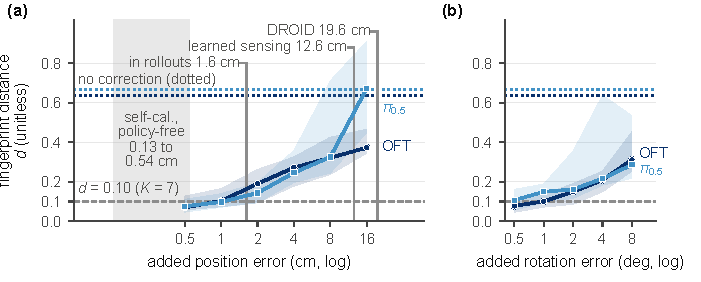
\includegraphics[width=0.92\linewidth]{figs/tolerance.pdf}
\caption{Policy sensitivity to imposed camera-pose error, with observed calibration-error regimes shown for comparison.}
\label{fig:tolerance}
\end{figure}

A separate rollout-free sensitivity analysis provides a scale for these errors. Both evaluated policy families begin to
depart noticeably from their training behavior at approximately 1--2 cm and $1^\circ$ of camera-pose error
(Fig.~\ref{fig:tolerance}), whereas successful self-calibration lies between 0.07 and 0.54 cm. Among raw camera failures,
self-measured coverage predicts repair with AUROC 0.74 [0.64, 0.84] ($n=98$), compared with 0.52 for translation
magnitude and 0.66 for rotation magnitude. The same pattern appears on LIBERO-Plus level-5 tasks: the initial-state
servo repairs 32 of 33 failures, and coverage continues to rank camera repairability despite the benchmark grade being
constant (AUROC 0.75, $n=47$). These results separate geometric recoverability from generic task difficulty.

\subsection{Policy-Based Diagnostics}

\label{sec:policy}

We next ask whether the policy's own action field provides an independent signal of camera misalignment. The policy is
queried at seven end-effector positions known from proprioception, and a local opening-action field is fitted from the
resulting commands. If these actions were directed toward a common sub-goal, one could in principle triangulate that
point and use the residual as a measure of frame consistency. Empirically, however, this statistic achieves only
0.32--0.56 AUROC across the evaluated families. Proposition~\ref{prop:div} explains the failure: for OFT, the symmetric
part of the fitted action Jacobian has positive trace on 97\% of units, and the inferred fixed point lies behind the
gripper on 94\%. Near the start of an episode, the behavior-cloned policy therefore resembles a locally diverging field
rather than the contracting field assumed by stable dynamical-system formulations \citep{ncds}.
The same probes are more informative when treated as a behavioral fingerprint rather than as a geometric
triangulation. Comparing the seven candidate-frame actions with the corresponding actions under the training setup gives
AUROC 0.93 for OFT and 0.79 for $\pi_{0.5}$, compared with 0.57 and 0.68 from the opening action alone. As a
frame-selection rule, the fingerprint improves over always correcting only for $\pi_{0.5}$, where it preserves the raw
frame on all five episodes that correction would otherwise break and raises success from 0.81 to 0.86. The registered
comparison fails for base OpenVLA because that policy does not reproduce its own training reference within the frozen
threshold. Full fingerprint results are reported in Appendix~\ref{app:fingerprint}. Overall, these experiments suggest
that geometric repairability can be predicted more reliably than the downstream effect of a correction on an arbitrary
policy.

\section{Limitations}
\label{sec:limits}

The main policy experiments use simulator segmentation and depth as proxies for a robot mask and RGB-D sensing. The
tolerance study indicates that the downstream policies require approximately centimeter- and degree-level camera
calibration. Our learned-mask pipeline reaches 12.6 cm error on the same 30 camera tasks, and calibration on real DROID
frames reaches 19.6 cm (Appendix~\ref{app:droid}); both are outside the measured tolerance. Consistent with this gap,
learned sensing does not yet outperform the raw policy, yielding 12/30 successes compared with 13/30 for the raw policy
and 19/30 with simulator sensing. The simulator results should therefore be interpreted as establishing the sensing
accuracy required by the method rather than demonstrating a complete real-world deployment pipeline.
The policy evaluation is also limited to simulation, one benchmark family, and three policy families. DROID is used to
evaluate self-calibration and the ground-truth-free consistency check on real images, but it does not constitute a
real-robot policy evaluation. In addition, the invertibility term must be specified for each nuisance family represented
by the model. Unmodeled effects can therefore be absorbed into the wrong channel; focal-length changes provide one such
example (Appendix~\ref{app:extra}). Finally, active calibration currently takes approximately one minute, which makes
the method more suitable for occasional deployment-time recalibration than for frame-by-frame adaptation.

\section{Conclusion}

This work treats deployment robustness as a property of both the policy and the observation interface through which the
policy acts. When a deployment shift changes the observation process without changing the task, the relevant questions
are whether the shift can be estimated and whether its effect can be inverted with sufficient fidelity. The
recoverability score formalizes these requirements and predicts repairability across held-out policy families without
retraining the policy. The same self-measurements support effective corrections for initial-pose and camera shifts,
while the attribution experiments distinguish calibration error, irreversible loss of visual coverage, and residual
policy failure. The principal practical limitation is sensing accuracy: deployment calibration must fall within the
downstream policy's tolerance. These results indicate that explicit measurement of the deployment interface can
complement policy-centric robustness methods by identifying when adaptation is necessary and when a training-free
correction is sufficient.

\subsection*{AI use statement}

We used generative AI tools (large language model coding and writing assistants) to write and debug experiment code,
to recompute and cross-check the reported statistics from the logged result rows, to search for related work, and to
draft and edit text. A vision-language model is also part of one experiment, where it chooses robot mask regions on
DROID images (Appendix~\ref{app:droid}); there it is a method component. Every reported number was recomputed from the
released result rows with the analysis scripts, and every reference was checked against its arXiv, proceedings or
publisher record. We have reviewed all AI-assisted work and take responsibility for the final content of this paper,
including text, claims and artifacts produced with the aid of generative AI.

\subsection*{Reproducibility statement}

Every constant of the score, the fingerprint and the registered decision rules was written to a dated log before the
data that tests it existed, and each registered test is reported against that entry, whatever its outcome
(Appendix~\ref{app:prereg}). Proofs are in Appendix~\ref{app:proofs}. Code, the run notebooks and every result row will
be released.

\bibliography{refs}
\bibliographystyle{iclr2027_conference}

\appendix

\section{Registered tests and their outcomes}
\label{app:prereg}
Each test below was written to a dated log, with its constants and pass criteria, before any data that could test it
existed. Development-family (OFT) outcomes are descriptive; held-out outcomes are the test.

\begin{table}[h]
\centering\small
\resizebox{\linewidth}{!}{%
\begin{tabular}{p{3.6cm}p{5.2cm}p{5.6cm}}
\toprule
test (registered) & rule & outcome \\
\midrule
Recoverability score as a predictor (frozen 2026-09-17) & rank raw failures by $\recover$ & \textbf{passes} on both
held-out families: 0.809 ($\pi_{0.5}$), 0.675 (base OpenVLA); category label 0.515, 0.472 \\
Do-no-harm gate (2026-09-18) & veto a correction if the action changes more under benign jitters of the corrected frame
than of the raw one & \textbf{fails}: over 386 paired gated / ungated units on the two held-out families it vetoed 49,
saved 1 unit and broke 16 ($p = 3\times10^{-4}$); where it does not veto it reproduces the ungated arm exactly \\
Score-gated correction (2026-09-19) & correct the camera only if coverage $\ge 0.5$ & \textbf{killed} by its own
criterion on rows unseen when frozen: prevented 2 breaks, gave up 3 repairs \\
Ray-concurrency probe (2026-09-19) & triangulate a sub-goal from 7 probe actions & \textbf{fails} on both families
(AUROC 0.32 to 0.56); explained by Prop.~\ref{prop:div} \\
Action-field fingerprint, H-F1 to H-F5 (amendment, 2026-09-19, before any held-out probe) & H-F1 corrected AUROC
$\ge 0.80$; H-F2 raw AUROC $\ge 0.70$; H-F3 keep raw on $\ge$ half the units a correction breaks; H-F4 keep the
correction on $\ge 80\%$ of units it repairs; H-F5 selected success $\ge$ best fixed arm minus one unit & $\pi_{0.5}$:
H-F3 and H-F5 pass (5 of 5; 0.86 against 0.81), H-F1 0.787, H-F2 0.684, H-F4 7 of 9 narrowly fail. Base OpenVLA:
H-F1 0.643, H-F2 0.659, H-F4 3 of 13, H-F5 0.32 against 0.46 fail; H-F3 undetermined (one unit) \\
DROID self-calibration stop rule (written before the final calibration run) & stop if the median error on reliable references exceeds 30 cm &
\textbf{fired} (32.1 cm); the later mask change reaching 19.6 cm is post hoc (Appendix~\ref{app:droid}) \\
\bottomrule
\end{tabular}}
\end{table}

\section{Real images: DROID}
\label{app:droid}
\begin{figure}[h]
\centering
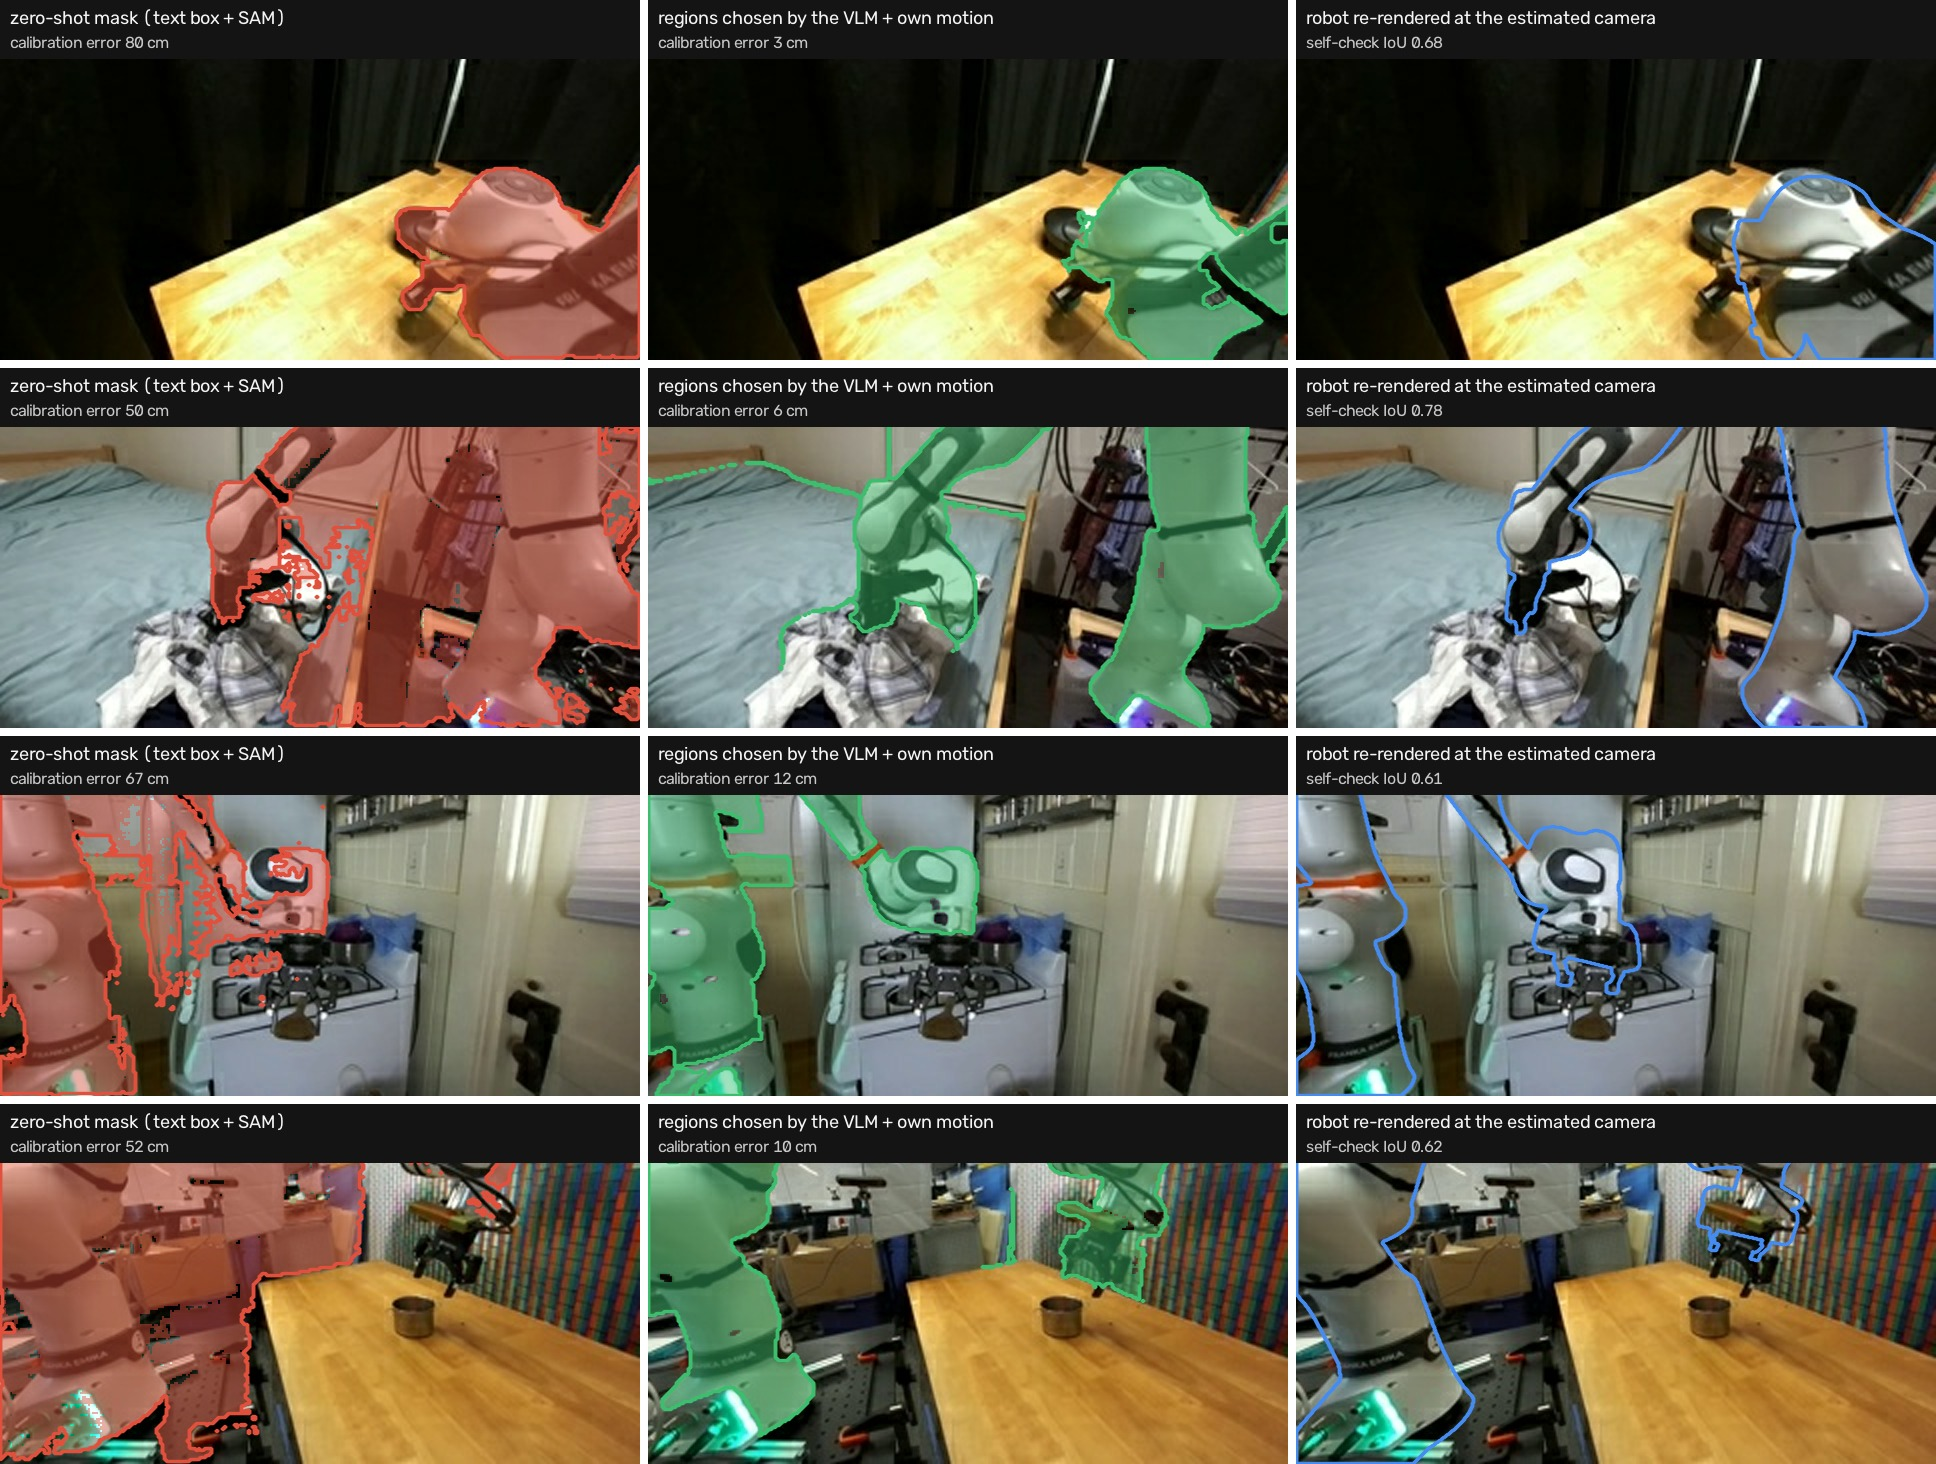
\includegraphics[width=\linewidth]{figs/droid_masks.jpg}
\caption{Real DROID frames. \textbf{Left:} a zero-shot text-box-plus-SAM mask attaches background to the robot, and a
silhouette calibration follows it. \textbf{Middle:} SAM regions chosen by a vision-language model, with part-robot
regions split by the robot's own motion. \textbf{Right:} the robot re-rendered at the estimated camera: the agreement is
a check the robot can run with no ground truth.}
\label{fig:droid}
\end{figure}

\begin{table}[h]
\centering\small
\caption{Self-calibration on 53 real DROID cameras; identical search, only the mask differs. The mask was changed after
the registered stop rule had fired on the first attempt (post hoc).}
\label{tab:droid}
\begin{tabular}{lcccc}
\toprule
& median error & under 30 cm & under 20 cm & paired Wilcoxon \\
\midrule
zero-shot masks & 25.4 cm / 25.1$^\circ$ & 28 & 19 & \\
VLM-chosen masks & \textbf{19.6 cm / 19.3$^\circ$} & 40 & 28 & $p=0.015$ \\
\bottomrule
\end{tabular}
\end{table}
Offline calibration of DROID from robot masks is not new \citep{caliball,poseddroid}. What we add is why the obvious
pipeline fails and what repairs it: completing a mask with frame-to-frame motion re-attaches moving background unless
motion is trusted only inside regions already called robot (precision 0.91 falls to 0.75 otherwise), and keeping the
largest connected component drops parts of an arm cut by the frame edge (recall 0.68 to 0.53 on one camera). The
ground-truth-free self-check correlates with the true error at $\rho=-0.40$ ($p=0.003$, $n=53$). A dedicated robot
segmenter \citep{robotseg} would be a natural third mask source; the comparison here holds the search fixed and varies
only the mask.

\section{Detailed Baseline Results}

\label{app:baselines}

The main text reports the aggregate comparison with test-time augmentation. Table~\ref{tab:baselines} gives the exact
30-task baseline counts used in that comparison.

\begin{table}[t]
\centering\small
\caption{Exact baseline results on 30 OFT \texttt{libero\_10} camera tasks.}
\label{tab:baselines}
\resizebox{0.85\linewidth}{!}{%
\begin{tabular}{lcccc}
\toprule
arm & success & repaired & broken & wrapper vs.\ arm (wins / losses, $p$) \\
\midrule
raw policy & 0.27 & & & \\
generic corrections (white balance, CLAHE, denoise) & 0.37 & 3/22 & 0/8 & 10 / 2, 0.039 \\
homography with our pose, no depth & 0.40 & 9/22 & 5/8 & 9 / 2, 0.065 \\
test-time augmentation & 0.47 & 6/22 & 0/8 & 8 / 3, 0.23 \\
\textbf{wrapper} & \textbf{0.63} & 13/22 & 2/8 & \\
\bottomrule
\end{tabular}}
\end{table}

\section{Action-Field Fingerprint Results}

\label{app:fingerprint}

Table~\ref{tab:fp} reports the complete action-field fingerprint results for the development policy and both held-out
families.

\begin{table}[t]
\centering\small
\caption{Action-field fingerprint results. All constants were fixed on OFT before held-out evaluation.}
\label{tab:fp}
\resizebox{\linewidth}{!}{%
\begin{tabular}{lccc}
\toprule
& OFT (dev.) & $\pi_{0.5}$ (held out) & base OpenVLA (held out) \\
\midrule
AUROC, corrected-frame distance predicts wrapped success & 0.928 & 0.787 & 0.643 \\
\quad the same from the opening action alone (no probes) & 0.571 & 0.679 & 0.693 \\
raw / wrapped / \textbf{fingerprint} / oracle & 0.70 / 0.84 / 0.80 / 0.90 & 0.70 / 0.81 / \textbf{0.86} / 0.90 & 0.13 / 0.46 / 0.32 / 0.48 \\
units a correction broke, kept raw & 0 of 1 & \textbf{5 of 5} & 0 of 1 \\
\bottomrule
\end{tabular}}
\end{table}

\section{Additional results and figures}
\label{app:extra}
\begin{table}[h]
\centering\small
\caption{The first score test, three base tasks per family (the setting in which the score was first frozen).}
\begin{tabular}{lcccc}
\toprule
& units & repaired & AUROC, score & AUROC, label \\
\midrule
OpenVLA-OFT (development) & 21 & 14 & 0.908 [0.68, 1.00] & 0.500 \\
$\pi_{0.5}$ (held out) & 21 & 14 & 0.837 [0.64, 1.00] & 0.464 \\
pooled & 42 & 28 & 0.881 [0.76, 0.98] & 0.482 \\
\bottomrule
\end{tabular}
\end{table}

\textbf{Rollout noise on $\pi_{0.5}$.} Across the three replicated runs of Sec.~\ref{sec:undo}, the outcome of a task
changes between runs on 10\% of camera tasks under the raw policy and 33\% under the measuring wrapper, the arm-motion
mechanism of Sec.~\ref{sec:cost} seen as variance. On the 10 light tasks run alongside, the measuring wrapper breaks
13 of 26 raw successes and repairs 3 ($p=0.021$); the motion-free arm of Sec.~\ref{sec:cost} breaks 1 of 54 light
successes on the ten-task sweep.

\textbf{A nuisance the body does not model.} Zooming the true camera while the wrapper assumes the training focal
length (8 camera tasks, policy-free) is absorbed as a camera that backed away along its own optical axis: at 5, 10 and
20\% zoom the pose error is 2.7, 5.9 and 10.8 cm, almost all of it along that axis. The corrected frame degrades
gracefully (image error 14.5, 16.3 and 20.1 against about 30 uncorrected and 10.2 with the true focal length), and the
self-check barely notices (F1 0.93 to 0.83): it verifies the pose it was asked about, not the model behind it. Focal
length is not aliased with the 6-DoF pose (Jacobian residual 0.78 against a median of 0.51 among the pose columns), so
three poses at different depths identify it; lens shift in $x$ is aliased with a 0.44 degree pan, which undoes it.

\begin{figure}[h]
\centering
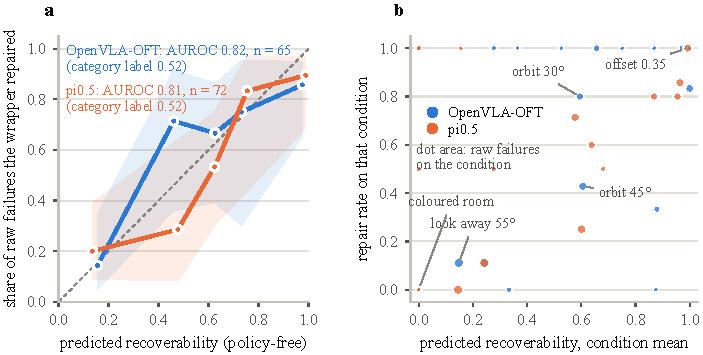
\includegraphics[width=1.0\linewidth]{figs/_unused/score.pdf}
\caption{Observed repair rate against the policy-free score, binned with Wilson bands (a), and per condition (b).}
\label{fig:score}
\end{figure}
\begin{figure}[h]
\centering
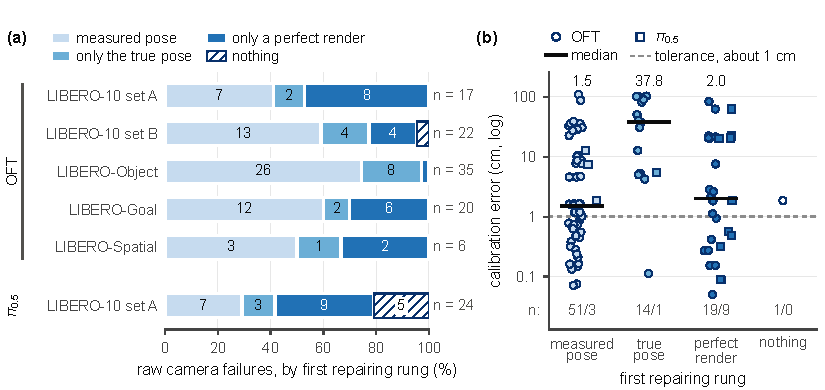
\includegraphics[width=1.0\linewidth]{figs/ladder.pdf}
\caption{(a) Every raw camera failure attributed to the first arm that repairs it; pooled over OFT, 1 of 100 belongs
to the policy. (b) The calibration error per bucket: only-true-pose units are gross calibration failures (median 38 cm),
only-render units were calibrated to 2 cm and lost the view.}
\label{fig:ladder}
\end{figure}
\begin{figure}[h]
\centering
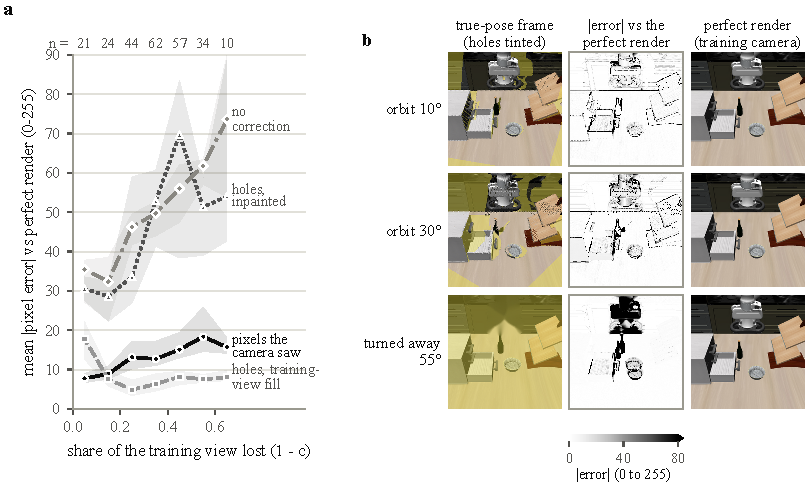
\includegraphics[width=0.6\linewidth]{figs/fidelity.pdf}
\caption{Error against a perfect training-view render on the 264 placements, split into seen pixels and holes, as a
function of the view lost (Prop.~\ref{prop:cov}). With a training-view fill the holes are cheap (median 7.6); the error
that grows with lost view sits on the seen pixels.}
\label{fig:fidelity}
\end{figure}
\begin{figure}[h]
\centering
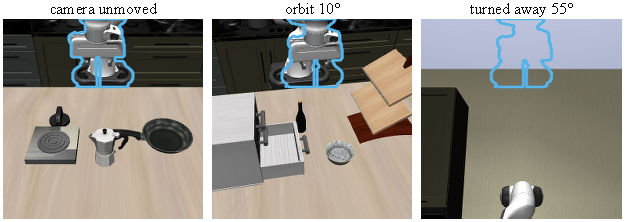
\includegraphics[width=1.0\linewidth]{figs/static_check.pdf}
\caption{The motion-free test of Prop.~\ref{prop:static}: the silhouette the training camera predicts (aqua) over the
deployed frame. When the camera has not moved it lands on the arm and the sweep is skipped.}
\label{fig:static}
\end{figure}
\begin{figure}[h]
\centering
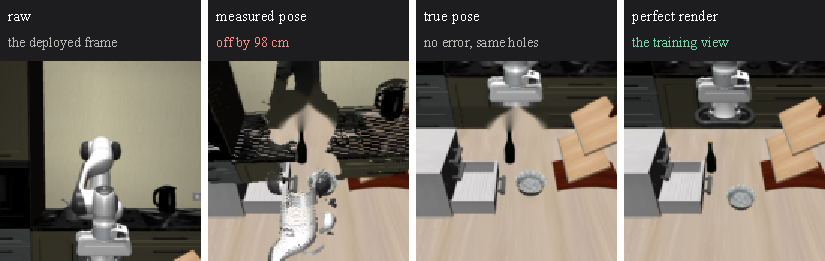
\includegraphics[width=1.0\linewidth]{figs_v2/ladder_pictures.pdf}
\caption{The ladder on one task (camera turned away 35 degrees): the measured pose fails (98 cm), the true pose still
leaves holes, only the training camera's own view has none.}
\label{fig:ladderpics}
\end{figure}
\begin{figure}[h]
\centering
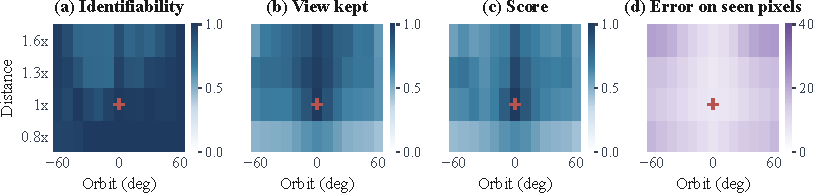
\includegraphics[width=1.0\linewidth]{figs_v2/figA_maps.pdf}
\caption{Policy-free maps over camera placements (means over three base tasks): identifiability, view kept, the score,
and the seen-pixel error after a true-pose re-rendering.}
\label{fig:maps}
\end{figure}
\begin{figure}[h]
\centering
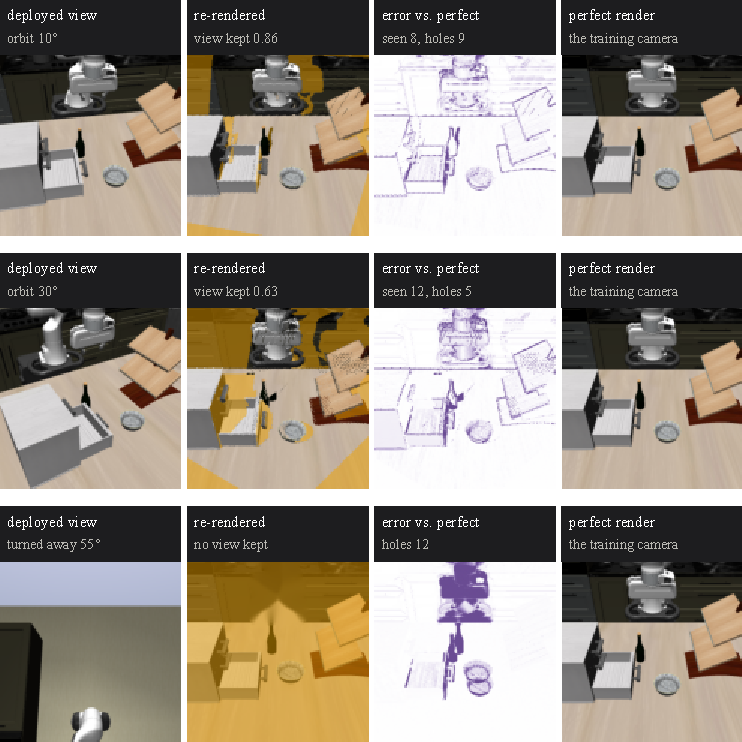
\includegraphics[width=0.9\linewidth]{figs_v2/fidelity_pictures.pdf}
\caption{Where the corrected frame is wrong, in pictures: holes (yellow) are filled cheaply; the error sits on seen
surfaces and grows with the orbit.}
\label{fig:fidpics}
\end{figure}
\begin{figure}[h]
\centering
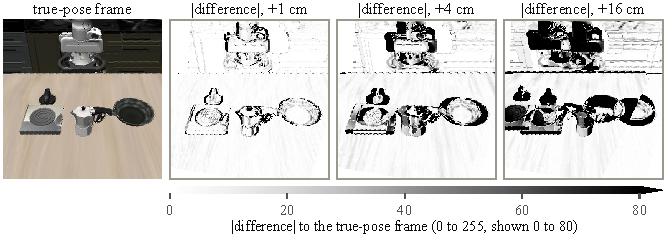
\includegraphics[width=1.0\linewidth]{figs/tolerance_pictures.pdf}
\caption{The frame handed to the policy when the true camera pose is perturbed by 1, 4 and 16 cm.}
\label{fig:tolpics}
\end{figure}

\section{Proofs}
\label{app:proofs}
\paragraph{Proposition~\ref{prop:cr}.} Linearise $z(q_k, \eta)$ about the true $\eta$: $z_k = z(q_k,\eta) + J_k
\delta + \epsilon_k$ with $\epsilon_k \sim (0, \sigma^2 I)$ independent. Stacking gives a linear Gaussian model with
Fisher information $\sigma^{-2} J^\top J$. The Cram\'er--Rao bound gives $\mathrm{Cov}(\hat\eta) \succeq \sigma^2
(J^\top J)^{-1}$, so $\mathbb{E}\|\hat\eta-\eta\|^2 \ge \sigma^2 \mathrm{tr}((J^\top J)^{-1}) \ge \sigma^2
\lambda_{\max}((J^\top J)^{-1}) = \sigma^2/\sigma_{\min}(J)^2$. Appending rows to $J$ appends a positive semidefinite
term to $J^\top J$, and by Weyl's inequality its smallest eigenvalue cannot decrease. The bound is first order; the
calibration we run also uses depth, which adds rows to $J$ and can only tighten it. (Measured with the full excursion of
the 7-pose sweep; halving the excursion gives 1.01 to 3.23 and 0.54 to 0.18 cm.)

\paragraph{Proposition~\ref{prop:cov}.} Split $\Omega = V \cup (\Omega\setminus V)$. A pixel $u \notin V$ has no
pre-image in the deployed frame $o_d$, so $o_{\mathrm{train}}(u)$ and $o_d$ are conditionally independent given the
scene prior, and any $\hat o(u) = f(o_d)$ has the Bayes risk of the best predictor from the prior alone,
$e_{\mathrm{prior}}(u)$. Summing over $\Omega\setminus V$ and adding the resampling error on $V$ gives the bound.

\paragraph{Proposition~\ref{prop:static}.} With $\eta = \eta_0$ and an exact body model, the rendered and observed
silhouettes are the same function of $q$, so $r(q) = d(\text{noise})$. If $r(q)$ exceeds what noise alone produces, the
premise fails. The test is one-sided: a zero residual at one pose is consistent with a small set of poses that project
the arm identically at that $q$, which is why the method measures with several poses once the test fires.

\paragraph{Proposition~\ref{prop:div}.} Under the triangulation model $a(p) = \lambda(g - p)$ the field's Jacobian is
$-\lambda I$ and $g$ its attracting fixed point. For the observed field $a(p) = 0$ at $g^\star = p_0 - A^{-1} a_0$, and
the flow $\dot p = a(p)$ linearised there has Jacobian $A$; if $\tfrac12(A + A^\top) \succ 0$ then $\tfrac{d}{dt}\|p -
g^\star\|^2 = 2 (p-g^\star)^\top A (p - g^\star) > 0$, so $g^\star$ repels. The least-squares triangulation returns
$g^\star$ regardless, and its residual measures the asymmetry of $A$, not the distance between the observation and the
training distribution.

\end{document}
